%!TeX root=../tempestrackham.tex
\Scene*{2}[The island. Before \textsc{Prospero's} cell.]



\begin{figure}[t]
	\centering
	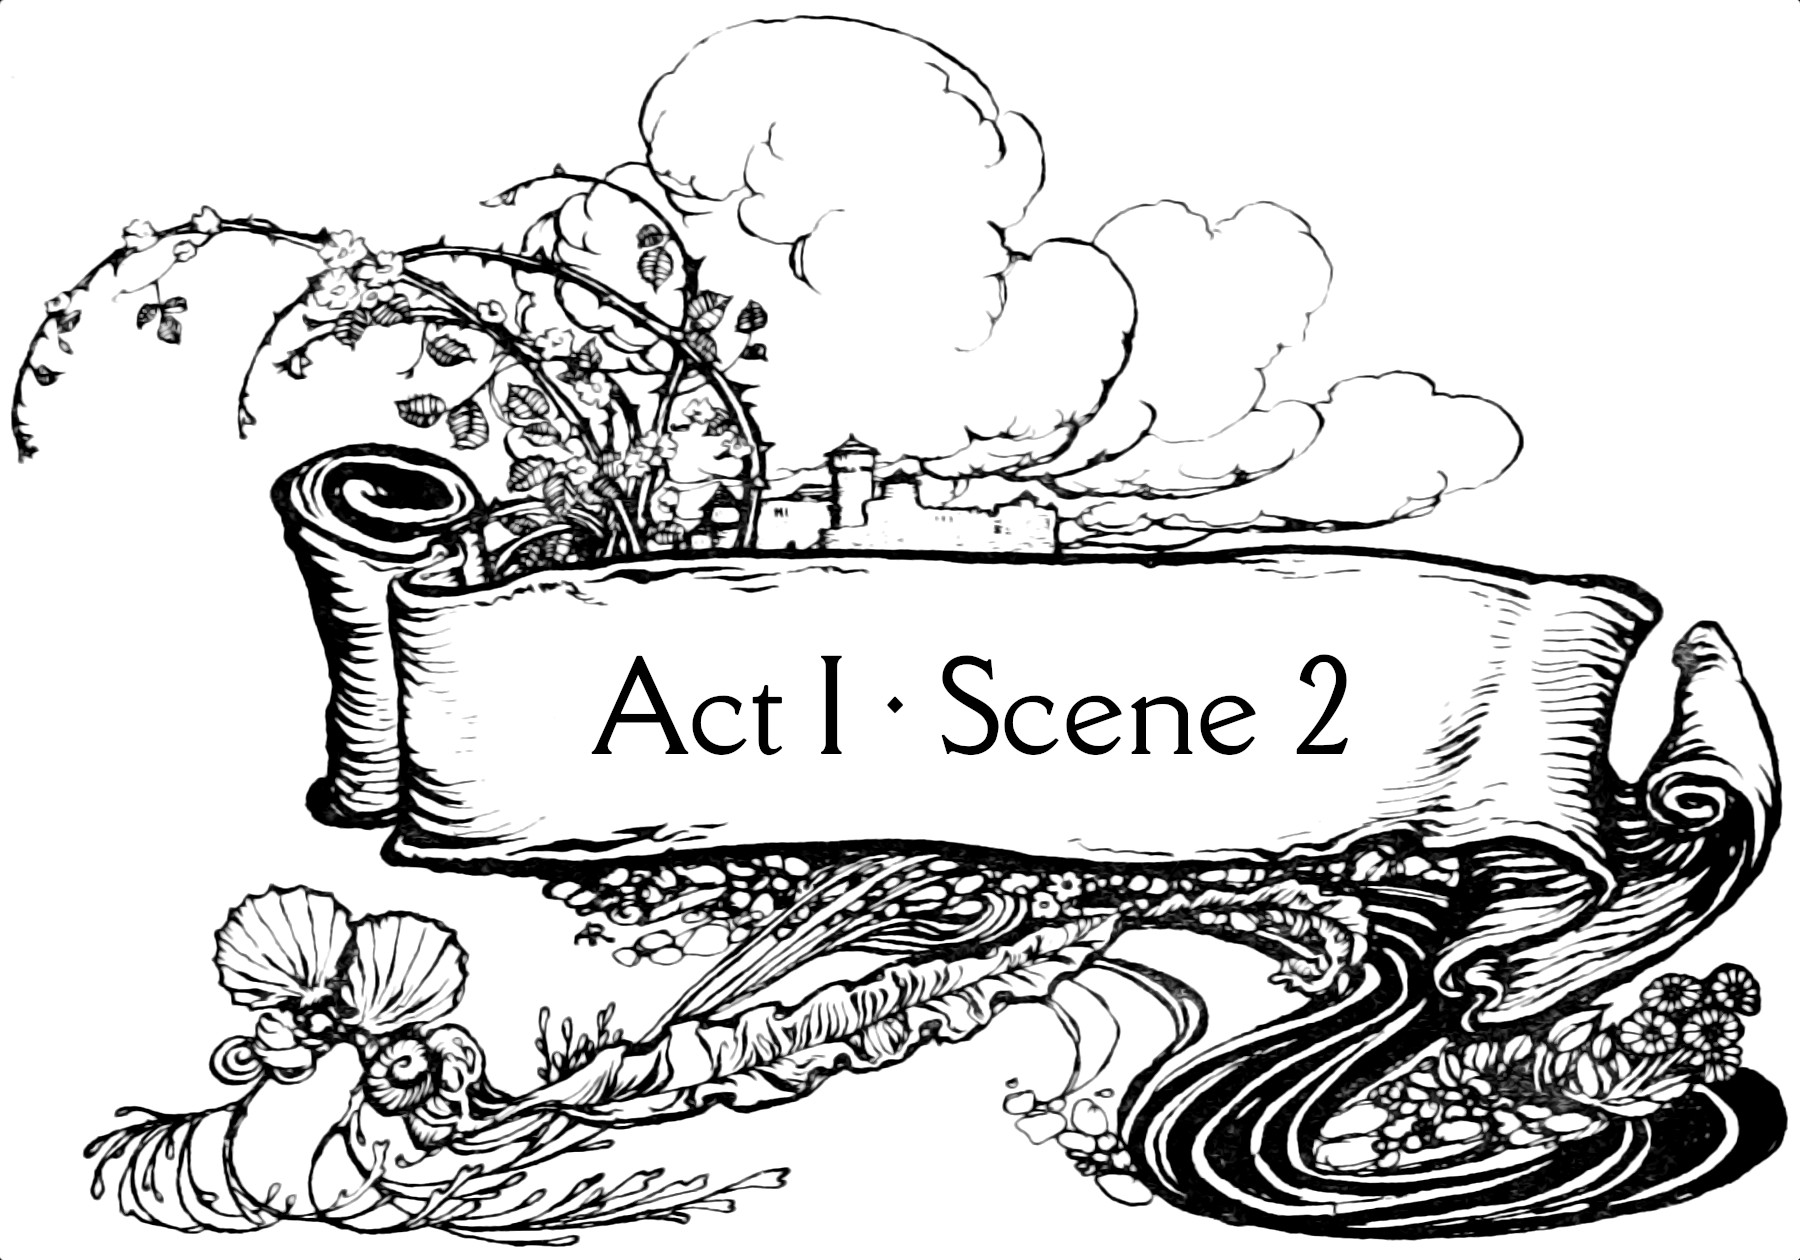
\includegraphics[width=\headerwidth]{1iihead}
\end{figure}


%\vspace{\textsink+1cm}


\textit{(The island. Before \textsc{Prospero's} cell.)}\centering

\begin{verse_speech}[Miranda] 
If by your art, my dearest father, you have\\
Put the wild waters in this roar, allay them.\\
The sky, it seems, would pour down stinking pitch,\\
But that the sea, mounting to the welkin's cheek,\\
Dashes the fire out. O, I have suffered\\
With those that I saw suffer: a brave vessel,\\
Who had, no doubt, some noble creature in her,\\
Dash'd all to pieces. O, the cry did knock\\
Against my very heart. Poor souls, they perish'd.\\
Had I been any god of power, I would\\
Have sunk the sea within the earth or ere\\
It should the good ship so have swallow'd and\\
The fraughting souls within her.\\
\end{verse_speech}


\begin{verse_speech}[Prospero] 
\hspace{\widthof{The fraughting souls within her.}}Be collected:\\
No more amazement: tell your piteous heart\\
There's no harm done.\\
\end{verse_speech}

\verseline[Miranda]{\hspace{\widthof{There's no harm done.}}O, woe the day!}
	
\begin{verse_speech}[Prospero] 
\hspace{\widthof{There's no harm done. O, woe the day!}}No harm.\\
I have done nothing but in care of thee,\\
Of thee, my dear one, thee, my daughter, who\\
Art ignorant of what thou art, nought knowing\\
Of whence I am, nor that I am more better\\
Than Prospero, master of a full poor cell,\\
And thy no greater father.
\end{verse_speech}

\begin{verse_speech}[Miranda] 
\hspace{\widthof{And thy no greater father.}}More to know\\
Did never meddle with my thoughts.
\end{verse_speech}

\begin{verse_speech}[Prospero] 
\hspace{\widthof{Did never meddle with my thoughts.}}'Tis time\\
I should inform thee farther. Lend thy hand,\\
And pluck my magic garment from me. So:\\
\stage{Lays down his mantle}
Lie there, my art. Wipe thou thine eyes; have comfort.\\
The direful spectacle of the wreck, which touch'd\\
The very virtue of compassion in thee,\\
I have with such provision in mine art\\
So safely ordered that there is no soul—\\
No, not so much perdition as an hair\\
Betid to any creature in the vessel\\
Which thou heard'st cry, which thou saw'st sink. Sit down;\\
For thou must now know farther.
\end{verse_speech}

\stage{They sit.}

\begin{verse_speech}[Miranda] 
\hspace{\widthof{For thou must now know farther.}}You have often\\
Begun to tell me what I am, but stopp'd\\
And left me to a bootless inquisition,\\
Concluding <Stay: not yet.>
\end{verse_speech}

\begin{verse_speech}[Prospero] 
\hspace{\widthof{Concluding <Stay: not yet.>}}The hour's now come;\\
The very minute bids thee ope thine ear;\\
Obey and be attentive. Canst thou remember\\
A time before we came unto this cell?\\
I do not think thou canst, for then thou wast not\\
Out three years old.
\end{verse_speech}


\verseline[Miranda]{\hspace{\widthof{Out three years old.}}Certainly, sir, I can.}
	
\begin{verse_speech}[Prospero] 
By what? by any other house or person?\\
Of any thing the image tell me that\\
Hath kept with thy remembrance.
\end{verse_speech}

\begin{verse_speech}[Miranda] 
\hspace{\widthof{Hath kept with thy remembrance.}}'Tis far off\\
And rather like a dream than an assurance\\
That my remembrance warrants. Had I not\\
Four or five women once that tended me?
\end{verse_speech}



\begin{pictures} % Miranda baby
	\begin{letter}
		\begin{colorbigpic}
			[1.1]
			{1ii_baby}
			{Thou wast not out three years old}
		\end{colorbigpic}
	\end{letter}

	\begin{a4}
		\begin{colorbigpic}
			[1]
			{1ii_baby}
			{Thou wast not out three years old}
		\end{colorbigpic}
	\end{a4}
\end{pictures}




\begin{verse_speech}[Prospero] 
Thou hadst, and more, Miranda. But how is it\\
That this lives in thy mind? What seest thou else\\
In the dark backward and abysm of time?\\
If thou remember'st aught ere thou camest here,\\
How thou camest here thou mayst.
\end{verse_speech}

\verseline[Miranda]{\hspace{\widthof{How thou camest here thou mayst.}}But that I do not.}

\begin{verse_speech}[Prospero] 
	Twelve year since, Miranda, twelve year since,\\
Thy father was the Duke of Milan and\\
A prince of power.
\end{verse_speech}

\verseline[Miranda]{\hspace{\widthof{A prince of power.}}Sir, are not you my father?}

\begin{verse_speech}[Prospero] 
Thy mother was a piece of virtue, and\\
She said thou wast my daughter; and thy father\\
Was Duke of Milan; and thou his only heir\\
And princess no worse issued.
\end{verse_speech}

\begin{verse_speech}[Miranda] 
\hspace{\widthof{And princess no worse issued.}}O the heavens!\\
What foul play had we, that we came from thence?\\
Or blessèd was't we did?
\end{verse_speech}

\begin{verse_speech}[Prospero] 
\hspace{\widthof{Or blessèd was't we did?}}Both, both, my girl:\\
By foul play, as thou say'st, were we heaved thence,\\
But blessedly holp hither.
\end{verse_speech}

\begin{verse_speech}[Miranda] 
\hspace{\widthof{But blessedly holp hither.}}O, my heart bleeds\\
To think o' the teen that I have turn'd you to,\\
Which is from my remembrance! Please you, farther.
\end{verse_speech}

\begin{verse_speech}[Prospero] 
My brother and thy uncle, call'd Antonio—\\
I pray thee, mark me—that a brother should\\
Be so perfidious!—he whom next thyself\\
Of all the world I loved and to him put\\
The manage of my state; as at that time\\
Through all the signories it was the first\\
And Prospero the prime duke, being so reputed\\
In dignity, and for the liberal arts\\
Without a parallel; those being all my study,\\
The government I cast upon my brother\\
And to my state grew stranger, being transported\\
And rapt in secret studies. Thy false uncle—\\
Dost thou attend me?
\end{verse_speech}

\verseline[Miranda]{\hspace{\widthof{Dost thou attend me?}}Sir, most heedfully.}
	
\begin{verse_speech}[Prospero] 
Being once perfected how to grant suits,\\
How to deny them, who to advance and who\\
To trash for over-topping, new created\\
The creatures that were mine, I say, or changed 'em,\\
Or else new form'd 'em; having both the key\\
Of officer and office, set all hearts i' the state\\
To what tune pleased his ear; that now he was\\
The ivy which had hid my princely trunk,\\
And suck'd my verdure out on't. Thou attend'st not.
\end{verse_speech}

\verseline[Miranda]{O, good sir, I do.}
	
\begin{verse_speech}[Prospero] 
\hspace{\widthof{O, good sir, I do.}}I pray thee, mark me.\\
I, thus neglecting worldly ends, all dedicated\\
To closeness and the bettering of my mind\\
With that which, but by being so retired,\\
O'er-prized all popular rate, in my false brother\\
Awaked an evil nature; and my trust,\\
Like a good parent, did beget of him\\
A falsehood in its contrary as great\\
As my trust was; which had indeed no limit,\\
A confidence sans bound. He being thus lorded,\\
Not only with what my revenue yielded,\\
But what my power might else exact, like one\\
Who having into truth, by telling of it,\\
Made such a sinner of his memory,\\
To credit his own lie, he did believe\\
He was indeed the duke; out o' the substitution\\
And executing the outward face of royalty,\\
With all prerogative: hence his ambition growing—\\
Dost thou hear?
\end{verse_speech}

\verseline[Miranda]{Your tale, sir, would cure deafness.}
	
\begin{verse_speech}[Prospero] 
To have no screen between this part he play'd\\
And him he play'd it for, he needs will be\\
Absolute Milan. Me, poor man, my library\\
Was dukedom large enough: of temporal royalties\\
He thinks me now incapable; confederates—\\
So dry he was for sway—wi' the King of Naples\\
To give him annual tribute, do him homage,\\
Subject his coronet to his crown and bend\\
The dukedom yet unbow'd—alas, poor Milan!—\\
To most ignoble stooping.
\end{verse_speech}

\verseline[Miranda]{\hspace{\widthof{To most ignoble stooping.}}O the heavens!}
	
\begin{verse_speech}[Prospero] 
Mark his condition and the event; then tell me\\
If this might be a brother.
\end{verse_speech}

\begin{verse_speech}[Miranda] 
\hspace{\widthof{If this might be a brother.}}I should sin\\
To think but nobly of my grandmother:\\
Good wombs have borne bad sons.
\end{verse_speech}

\begin{verse_speech}[Prospero] 
\hspace{\widthof{Good wombs have borne bad sons.}}Now the condition.\\
The King of Naples, being an enemy\\
To me inveterate, hearkens my brother's suit;\\
Which was, that he, in lieu o' the premises\\
Of homage and I know not how much tribute,\\
Should presently extirpate me and mine\\
Out of the dukedom and confer fair Milan\\
With all the honours on my brother: whereon,\\
A treacherous army levied, one midnight\\
Fated to the purpose did Antonio open\\
The gates of Milan, and, i' the dead of darkness,\\
The ministers for the purpose hurried thence\\
Me and thy crying self.
\end{verse_speech}

\begin{verse_speech}[Miranda] 
\hspace{\widthof{Me and thy crying self.}}Alack, for pity!\\
I, not remembering how I cried out then,\\
Will cry it o'er again: it is a hint\\
That wrings mine eyes to't.
\end{verse_speech}

\begin{verse_speech}[Prospero] 
\hspace{\widthof{That wrings mine eyes to't.}}Hear a little further\\
And then I'll bring thee to the present business\\
Which now's upon's; without the which this story\\
Were most impertinent.
\end{verse_speech}

\begin{verse_speech}[Miranda] 
\hspace{\widthof{Were most impertinent.}}Wherefore did they not\\
That hour destroy us?
\end{verse_speech}

\begin{verse_speech}[Prospero] 
\hspace{\widthof{That hour destroy us?}}Well demanded, wench:\\
My tale provokes that question. Dear, they durst not,\\
So dear the love my people bore me, nor set\\
A mark so bloody on the business, but\\
With colours fairer painted their foul ends.\\
In few, they hurried us aboard a bark,\\
Bore us some leagues to sea; where they prepared\\
A rotten carcass of a boat, not rigg'd,\\
Nor tackle, sail, nor mast; the very rats\\
Instinctively had quit it: there they hoist us,\\
To cry to the sea that roar'd to us, to sigh\\
To the winds whose pity, sighing back again,\\
Did us but loving wrong.
\end{verse_speech}

\begin{verse_speech}[Miranda] 
\hspace{\widthof{That hour destroy us?}}Alack, what trouble\\
Was I then to you!
\end{verse_speech}

\begin{verse_speech}[Prospero] 
\hspace{\widthof{Was I then to you!}}O, a cherubim\\
Thou wast that did preserve me. Thou didst smile.\\
Infusèd with a fortitude from heaven,\\
When I have deck'd the sea with drops full salt,\\
Under my burthen groan'd; which raised in me\\
An undergoing stomach, to bear up\\
Against what should ensue.
\end{verse_speech}

\verseline[Miranda]{How came we ashore?}
	
\begin{verse_speech}[Prospero] 
By Providence divine.\\
Some food we had and some fresh water that\\
A noble Neapolitan, Gonzalo,\\
Out of his charity, being then appointed\\
Master of this design, did give us, with\\
Rich garments, linens, stuffs and necessaries,\\
Which since have steaded much; so, of his gentleness,\\
Knowing I loved my books, he furnish'd me\\
From mine own library with volumes that\\
I prize above my dukedom.
\end{verse_speech}

\begin{verse_speech}[Miranda] 
\hspace{\widthof{I prize above my dukedom.}}Would I might\\
But ever see that man!
\end{verse_speech}


\begin{verse_speech}[Prospero] 
\hspace{\widthof{But ever see that man!}}Now I arise:\\
\stage{Stands and resumes his mantle}
Sit still, and hear the last of our sea-sorrow.\\
Here in this island we arrived; and here\\
Have I, thy schoolmaster, made thee more profit\\
Than other princesses can that have more time\\
For vainer hours and tutors not so careful.
\end{verse_speech}

\begin{verse_speech}[Miranda] 
Heavens thank you for't! And now, I pray you, sir,\\
For still 'tis beating in my mind, your reason\\
For raising this sea-storm?
\end{verse_speech}

\begin{verse_speech}[Prospero] 
\hspace{\widthof{For raising this sea-storm?}}Know thus far forth.\\
By accident most strange, bountiful Fortune,\\
Now my dear lady, hath mine enemies\\
Brought to this shore; and by my prescience\\
I find my zenith doth depend upon\\
A most auspicious star, whose influence\\
If now I court not but omit, my fortunes\\
Will ever after droop. Here cease more questions:\\
Thou art inclined to sleep; 'tis a good dullness,\\
And give it way: I know thou canst not choose.\\
\stage{\textsc{Miranda} sleeps}
Come away, servant, come. I am ready now.\\
Approach, my Ariel, come.\\
\end{verse_speech}
\enter{\textsc{Ariel}}

\begin{verse_speech}[Ariel] 
All hail, great master! grave sir, hail! I come\\
To answer thy best pleasure; be't to fly,\\
To swim, to dive into the fire, to ride\\
On the curl'd clouds, to thy strong bidding task\\
Ariel and all his quality.
\end{verse_speech}

\begin{verse_speech}[Prospero] 
\hspace{\widthof{Ariel and all his quality.}}Hast thou, spirit,\\
Perform'd to point the tempest that I bade thee?
\end{verse_speech}

\begin{verse_speech}[Ariel] 
To every article.\\
I boarded the king's ship; now on the beak,\\
Now in the waist, the deck, in every cabin,\\
I flamed amazement: sometime I'ld divide,\\
And burn in many places; on the topmast,\\
The yards and bowsprit, would I flame distinctly,\\
Then meet and join. Jove's lightnings, the precursors\\
O' the dreadful thunder-claps, more momentary\\
And sight-outrunning were not; the fire and cracks\\
Of sulphurous roaring the most mighty Neptune\\
Seem to besiege and make his bold waves tremble,\\
Yea, his dread trident shake.
\end{verse_speech}

\begin{verse_speech}[Prospero] 
\hspace{\widthof{Yea, his dread trident shake.}}My brave spirit!\\
Who was so firm, so constant, that this coil\\
Would not infect his reason?
\end{verse_speech}

\begin{verse_speech}[Ariel] 
\hspace{\widthof{Would not infect his reason?}}Not a soul\\
But felt a fever of the mad and play'd\\
Some tricks of desperation. All but mariners\\
Plunged in the foaming brine and quit the vessel,\\
Then all afire with me: the king's son, Ferdinand,\\
With hair up-staring,—then like reeds, not hair,—\\
Was the first man that leap'd; cried, <Hell is empty\\
And all the devils are here.>
\end{verse_speech}

\begin{letter}
	\enlargethispage{\baselineskip}
\end{letter}

\begin{verse_speech}[Prospero] 
\hspace{\widthof{And all the devils are here.}}Why that's my spirit!\\
But was not this nigh shore?
\end{verse_speech}

\verseline[Ariel]{\hspace{\widthof{But was not this nigh shore?}}Close by, my master.}

\begin{pictures} % ship in harbor - letter
	\begin{letter}
		\begin{colorbigpic}
			[1.1]
			{1ii_harbor}
			{Safely in harbour is the king's ship}
		\end{colorbigpic}
	\end{letter}
\end{pictures}


	
\verseline[Prospero]{But are they, Ariel, safe?}
	
\begin{verse_speech}[Ariel] 
\hspace{\widthof{But are they, Ariel, safe?}}Not a hair perish'd;\\
On their sustaining garments not a blemish,\\
But fresher than before: and, as thou badest me,\\
In troops I have dispersed them 'bout the isle.\\
The king's son have I landed by himself;\\
Whom I left cooling of the air with sighs\\
In an odd angle of the isle and sitting,\\
His arms in this sad knot.
\end{verse_speech}
\stage{He folds his arms.}

\begin{verse_speech}[Prospero] 
\hspace{\widthof{His arms in this sad knot.}}Of the king's ship\\
The mariners say how thou hast disposed\\
And all the rest o' the fleet.
\end{verse_speech}



\begin{pictures} % ship in harbor - a4
	\begin{a4}
		\begin{colorbigpic}
			[1]
			{1ii_harbor}
			{Safely in harbour is the king's ship}
		\end{colorbigpic}
	\end{a4}
\end{pictures}
	



\begin{verse_speech}[Ariel] 
\hspace{\widthof{And all the rest o' the fleet.}}Safely in harbour\\
Is the king's ship; in the deep nook, where once\\
Thou call'dst me up at midnight to fetch dew\\
From the still-vex'd Bermoothes, there she's hid:\\
The mariners all under hatches stow'd;\\
Who, with a charm join'd to their suffer'd labour,\\
I have left asleep; and for the rest o' the fleet\\
Which I dispersed, they all have met again\\
And are upon the Mediterranean flote,\\
Bound sadly home for Naples,\\
Supposing that they saw the king's ship wreck'd\\
And his great person perish.
\end{verse_speech}

\begin{verse_speech}[Prospero] 
\hspace{\widthof{And his great person perish.}}Ariel, thy charge\\
Exactly is perform'd: but there's more work.\\
What is the time o' the day?
\end{verse_speech}

\verseline[Ariel]{\hspace{\widthof{What is the time o' the day?}}Past the mid season.}

\begin{verse_speech}[Prospero] 
At least two glasses. The time 'twixt six and now\\
Must by us both be spent most preciously.
\end{verse_speech}

\begin{verse_speech}[Ariel] 
Is there more toil? Since thou dost give me pains,\\
Let me remember thee what thou hast promised,\\
Which is not yet perform'd me.
\end{verse_speech}

\begin{verse_speech}[Prospero] 
\hspace{\widthof{Which is not yet perform'd me.}}How now? moody?\\
What is't thou canst demand?
\end{verse_speech}

\verseline[Ariel]{\hspace{\widthof{What is't thou canst demand?}}My liberty.}

\verseline[Prospero]{Before the time be out? no more!}
	
\begin{verse_speech}[Ariel] 
\hspace{\widthof{Before the time be out? no more!}}I prithee,\\
Remember I have done thee worthy service;\\
Told thee no lies, made thee no mistakings, served\\
Without or grudge or grumblings: thou didst promise\\
To bate me a full year.
\end{verse_speech}



\begin{pictures} % Sycorax portrait - letter
	\begin{letter}
		\begin{colorbigpic}
			[1.1]
			{1ii_sycorax}
			{The foul witch Sycorax}
		\end{colorbigpic}
	\end{letter}

\end{pictures}



\begin{verse_speech}[Prospero] 
\hspace{\widthof{To bate me a full year.}}Dost thou forget\\
From what a torment I did free thee?
\end{verse_speech}

\verseline[Ariel]{\hspace{\widthof{From what a torment I did free thee?}}No.}
	
\begin{verse_speech}[Prospero] 
Thou dost, and think'st it much to tread the ooze\\
Of the salt deep,\\
To run upon the sharp wind of the north,\\
To do me business in the veins o' the earth\\
When it is baked with frost.
\end{verse_speech}

\verseline[Ariel]{\hspace{\widthof{When it is baked with frost.}}I do not, sir.}



\begin{pictures} % Sycorax portrait - a4
	\begin{a4}
		\begin{colorbigpic}
			[1]
			{1ii_sycorax}
			{The foul witch Sycorax}
		\end{colorbigpic}
	\end{a4}
\end{pictures}



\begin{verse_speech}[Prospero] 
Thou liest, malignant thing! Hast thou forgot\\
The foul witch Sycorax, who with age and envy\\
Was grown into a hoop? hast thou forgot her?
\end{verse_speech}

\verseline[Ariel]{No, sir.}

	
\verseline[Prospero]{Thou hast. Where was she born? speak; tell me.}
	
\verseline[Ariel]{Sir, in Argier.}

\begin{letter}
	\begin{figure}[tb]
		\centering
		
\includegraphics[width=\textwidth]{grotesque}
	\end{figure}
\end{letter}
	
\begin{verse_speech}[Prospero] 
\hspace{\widthof{Sir, in Argier.}}O, was she so? I must\\
Once in a month recount what thou hast been,\\
Which thou forget'st. This damn'd witch Sycorax,\\
For mischiefs manifold and sorceries terrible\\
To enter human hearing, from Argier,\\
Thou know'st, was banish'd: for one thing she did\\
They would not take her life. Is not this true?
\end{verse_speech}

\verseline[Ariel]{Ay, sir.}

\begin{verse_speech}[Prospero] 
This blue-eyed hag was hither brought with child\\
And here was left by the sailors. Thou, my slave,\\
As thou report'st thyself, wast then her servant;\\
And, for thou wast a spirit too delicate\\
To act her earthy and abhorr'd commands,\\
Refusing her grand hests, she did confine thee,\\
By help of her more potent ministers\\
And in her most unmitigable rage,\\
Into a cloven pine; within which rift\\
Imprison'd thou didst painfully remain\\
A dozen years; within which space she died\\
And left thee there; where thou didst vent thy groans\\
As fast as mill-wheels strike. Then was this island—\\
Save for the son that she did litter here,\\
A freckled whelp hag-born—not honour'd with\\
A human shape.
\end{verse_speech}


\begin{pictures} % cloven pine - letter
	\begin{letter}
		\begin{colorbigpic}
			[1]
			{1ii_clovenpine}
			{She did confine thee\dots into a cloven pine}
		\end{colorbigpic}
	\end{letter}
\end{pictures}



\verseline[Ariel]{\hspace{\widthof{A human shape.}}Yes, Caliban her son.}
	
\begin{verse_speech}[Prospero] 
Dull thing, I say so; he, that Caliban\\
Whom now I keep in service. Thou best know'st\\
What torment I did find thee in; thy groans\\
Did make wolves howl and penetrate the breasts\\
Of ever angry bears: it was a torment\\
To lay upon the damn'd, which Sycorax\\
Could not again undo: it was mine art,\\
When I arrived and heard thee, that made gape\\
The pine and let thee out.
\end{verse_speech}

\verseline[Ariel]{\hspace{\widthof{The pine and let thee out.}}I thank thee, master.}
	
\begin{verse_speech}[Prospero] 
If thou more murmur'st, I will rend an oak\\
And peg thee in his knotty entrails till\\
Thou hast howl'd away twelve winters.
\end{verse_speech}



\begin{pictures} % cloven pine - a4
	\begin{a4}
		\begin{colorbigpic}
			[1]
			{1ii_clovenpine}
			{She did confine thee\dots into a cloven pine}
		\end{colorbigpic}
	\end{a4}
\end{pictures}



\begin{verse_speech}[Ariel] 
\hspace{\widthof{Thou hast howl'd away twelve winters.}}Pardon, master;\\
I will be correspondent to command\\
And do my spiriting gently.
\end{verse_speech}

\begin{verse_speech}[Prospero] 
\hspace{\widthof{And do my spiriting gently.}}Do so, and after two days\\
I will discharge thee.
\end{verse_speech}

\begin{verse_speech}[Ariel] 
\hspace{\widthof{I will discharge thee.}}That's my noble master!\\
What shall I do? say what; what shall I do?
\end{verse_speech}


\begin{pictures} % Ariel like a water-nymph - letter
	\begin{letter}
		\begin{colorbigpic}
			[1.1]
			{1ii_waternymph}
			{Ariel like a water-nymph}
		\end{colorbigpic}
	\end{letter}
\end{pictures}


\begin{verse_speech}[Prospero] 
Go make thyself like a nymph o' the sea: be subject\\
To no sight but thine and mine, invisible\\
To every eyeball else. Go take this shape\\
And hither come in't: go, hence with diligence!\\
\exit{\textsc{Ariel}}
Awake, dear heart, awake! thou hast slept well; \\
Awake!
\end{verse_speech}

\begin{verse_speech}[Miranda] 
\hspace{\widthof{Awake!}}The strangeness of your story put\\
Heaviness in me.
\end{verse_speech}

\begin{verse_speech}[Prospero] 
\hspace{\widthof{Heaviness in me.}}Shake it off. Come on;\\
We'll visit Caliban my slave, who never\\
Yields us kind answer.
\end{verse_speech}

\begin{verse_speech}[Miranda] 
\hspace{\widthof{Yields us kind answer.}}'Tis a villain, sir,\\
I do not love to look on.
\end{verse_speech}


\begin{pictures} % Ariel like a water-nymph - a4
	\begin{a4}
		\begin{colorbigpic}
			[1.0]
			{1ii_waternymph}
			{Ariel like a water-nymph}
		\end{colorbigpic}
	\end{a4}
\end{pictures}



\begin{verse_speech}[Prospero] 
\hspace{\widthof{I do not love to look on.}}But, as 'tis,\\
We cannot miss him: he does make our fire,\\
Fetch in our wood and serves in offices\\
That profit us. What, ho! slave! Caliban!\\
Thou earth, thou! speak.
\end{verse_speech}

\begin{verse_speech}[Caliban]
\textit{[Within]} \hspace{\widthof{Thou earth, thou! speak.}-\widthof{[Within]}}There's wood enough within.
\end{verse_speech}

\begin{verse_speech}[Prospero] 
Come forth, I say! there's other business for thee:\\
Come, thou tortoise! when?\\
\stage{Re-enter \textsc{Ariel} like a water-nymph}
Fine apparition! My quaint Ariel,\\
Hark in thine ear.
\end{verse_speech}

\stage{He whispers to \textsc{Ariel}.}


\verseline[Ariel]{\hspace{\widthof{Hark in thine ear.}}My lord, it shall be done.}
\exit{\textsc{Ariel}}

\begin{verse_speech}[Prospero] 
Thou poisonous slave, got by the devil himself\\
Upon thy wicked dam, come forth!
\end{verse_speech}
\enter{\textsc{Caliban}}

\begin{verse_speech}[Caliban] 
As wicked dew as e'er my mother brush'd\\
With raven's feather from unwholesome fen\\
Drop on you both! a south-west blow on ye\\
And blister you all o'er!
\end{verse_speech}

\begin{verse_speech}[Prospero] 
For this, be sure, to-night thou shalt have cramps,\\
Side-stitches that shall pen thy breath up; urchins\\
Shall, for that vast of night that they may work,\\
All exercise on thee; thou shalt be pinch'd\\
As thick as honeycomb, each pinch more stinging\\
Than bees that made 'em.
\end{verse_speech}

\begin{verse_speech}[Caliban] 
\hspace{\widthof{Than bees that made 'em.}}I must eat my dinner.\\
This island's mine, by Sycorax my mother,\\
Which thou takest from me. When thou camest first,\\
Thou strokedst me and madest much of me, wouldst give me\\
Water with berries in't, and teach me how\\
To name the bigger light, and how the less,\\
That burn by day and night: and then I loved thee\\
And show'd thee all the qualities o' the isle,\\
The fresh springs, brine-pits, barren place and fertile:\\
Cursed be I that did so! All the charms\\
Of Sycorax, toads, beetles, bats, light on you!\\
For I am all the subjects that you have,\\
Which first was mine own king: and here you sty me\\
In this hard rock, whiles you do keep from me\\
The rest o' the island.
\end{verse_speech}

\begin{verse_speech}[Prospero] 
\hspace{\widthof{The rest o' the island.}}Thou most lying slave,\\
Whom stripes may move, not kindness! I have used thee,\\
Filth as thou art, with human care, and lodged thee\\
In mine own cell, till thou didst seek to violate\\
The honour of my child.
\end{verse_speech}

\begin{verse_speech}[Caliban]
O ho, O ho! would't had been done!\\
Thou didst prevent me; I had peopled else\\
This isle with Calibans.
\end{verse_speech}

\begin{verse_speech}[Miranda] 
\hspace{\widthof{This isle with Calibans.}}Abhorrèd slave,\\
Which any print of goodness wilt not take,\\
Being capable of all ill! I pitied thee,\\
Took pains to make thee speak, taught thee each hour\\
One thing or other: when thou didst not, savage,\\
Know thine own meaning, but wouldst gabble like\\
A thing most brutish, I endow'd thy purposes\\
With words that made them known. But thy vile race,\\
Though thou didst learn, had that in't which good natures\\
Could not abide to be with; therefore wast thou\\
Deservedly confined into this rock,\\
Who hadst deserved more than a prison.
\end{verse_speech}



\begin{verse_speech}[Caliban] 
You taught me language; and my profit on't\\
Is, I know how to curse. The red plague rid you\\
For learning me your language!
\end{verse_speech}

\begin{verse_speech}[Prospero] 
\hspace{\widthof{For learning me your language!}}Hag-seed, hence!\\
Fetch us in fuel; and be quick, thou'rt best,\\
To answer other business. Shrug'st thou, malice?\\
If thou neglect'st or dost unwillingly\\
What I command, I'll rack thee with old cramps,\\
Fill all thy bones with aches, make thee roar\\
That beasts shall tremble at thy din.
\end{verse_speech}


\begin{pictures} % Come unto these yellow sands - a4
	\begin{a4}
		\begin{colorbigpic}
			[1.0]
			{1ii_yellowsands}
			{Come unto these yellow sands}
		\end{colorbigpic}
	\end{a4}
\end{pictures}



\begin{verse_speech}[Caliban] 
\hspace{\widthof{That beasts shall tremble at thy din.}}No, pray thee.\\
\aside{I must obey: his art is of such power,\\
It would control my dam's god, Setebos,\\
And make a vassal of him.}
\end{verse_speech}

\begin{verse_speech}[Prospero] 
\hspace{\widthof{And make a vassal of him.}}So, slave; hence!
\end{verse_speech}

\exit{\textsc{Caliban}}

\begin{figure}[tb]
	\centering
	
\includegraphics[width=.45\textwidth]{batrider}
\end{figure}

\stage{Re-enter \textsc{Ariel}, invisible, playing and singing; \textsc{Ferdinand} following}


\begin{pictures} % Come unto these yellow sands - letter
	\begin{letter}
		\begin{colorbigpic}
			[1.1]
			{1ii_yellowsands}
			{Come unto these yellow sands}
		\end{colorbigpic}
	\end{letter}
\end{pictures}


\begin{song}[\textsc{Ariel's} song.]
	\songline{Come unto these yellow sands,}
	\songline{And then take hands:}
	\songline{Courtsied when you have and kiss'd}
	\songline{The wild waves whist,}
	\songline{Foot it featly here and there;}
	\songline{And, sweet sprites, the burthen bear.}
	\songline{Hark, hark!}
	\refrain{Bow-wow}
	\songline{The watch-dogs bark!}
	\refrain{Bow-wow}
	\songline{Hark, hark! I hear}
	\songline{The strain of strutting chanticleer}
	\songline{Cry, Cock-a-diddle-dow.}
\end{song}

\begin{verse_speech}[Ferdinand] 
Where should this music be? i' the air or the earth?\\
It sounds no more: and sure, it waits upon\\
Some god o' the island. Sitting on a bank,\\
Weeping again the king my father's wreck,\\
This music crept by me upon the waters,\\
Allaying both their fury and my passion\\
With its sweet air: thence I have follow'd it,\\
Or it hath drawn me rather. But 'tis gone.\\
No, it begins again.
\stage{\textsc{Ariel} sings}
\begin{song}
\songline{Full fathom five thy father lies;}
\songline{Of his bones are coral made;}
\songline{Those are pearls that were his eyes:}
\songline{Nothing of him that doth fade}
\songline{But doth suffer a sea-change}
\songline{Into something rich and strange.}
\songline{Sea-nymphs hourly ring his knell}
\refrain{Ding-dong}
\songline{Hark! now I hear them,—}
\refrain{Ding-dong, bell.}
\end{song}
\end{verse_speech}


\begin{verse_speech}[Ferdinand] 
The ditty does remember my drown'd father.\\
This is no mortal business, nor no sound\\
That the earth owes. I hear it now above me.\\
\end{verse_speech}

\begin{verse_speech}[Prospero] 
The fringèd curtains of thine eye advance\\
And say what thou seest yond.
\end{verse_speech}

\begin{verse_speech}[Miranda] 
\hspace{\widthof{And say what thou seest yond.}}What is't? a spirit?\\
Lord, how it looks about! Believe me, sir,\\
It carries a brave form. But 'tis a spirit.
\end{verse_speech}


\begin{pictures} % Where should this music be? - a4
	\begin{a4}
		\begin{colorbigpic}
			[1.0]
			{1ii_ferdmusic}
			{Where should this music be? i' the air or the earth?}
		\end{colorbigpic}
	\end{a4}
\end{pictures}
	


\begin{verse_speech}[Prospero] 
No, wench; it eats and sleeps and hath such senses\\
As we have, such. This gallant which thou seest\\
Was in the wreck; and, but he's something stain'd\\
With grief that's beauty's canker, thou mightst call him\\
A goodly person: he hath lost his fellows\\
And strays about to find 'em.
\end{verse_speech}

\begin{verse_speech}[Miranda] 
\hspace{\widthof{And strays about to find 'em.}}I might call him\\
A thing divine, for nothing natural\\
I ever saw so noble.
\end{verse_speech}



\begin{pictures} % Where should this music be? - letter
	\begin{letter}
		\begin{colorbigpic}
			[1.1]
			{1ii_ferdmusic}
			{Where should this music be? i' the air or the earth?}
		\end{colorbigpic}
	\end{letter}
\end{pictures}
	



\begin{verse_speech}[Prospero]\aside{\hspace{\widthof{I ever saw so noble.}-\widthof{[Aside]}}It goes on, I see,\\
As my soul prompts it. Spirit, fine spirit! I'll free thee\\
Within two days for this.}
\end{verse_speech}

\begin{verse_speech}[Ferdinand] 
\hspace{\widthof{Within two days for this.}}Most sure, the goddess\\
On whom these airs attend! Vouchsafe my prayer\\
May know if you remain upon this island;\\
And that you will some good instruction give\\
How I may bear me here: my prime request,\\
Which I do last pronounce, is, O you wonder!\\
If you be maid or no?
\end{verse_speech}

\begin{verse_speech}[Miranda] 
\hspace{\widthof{If you be maid or no?}}No wonder, sir;\\
But certainly a maid.
\end{verse_speech}

\begin{figure}[tb]
	\centering
	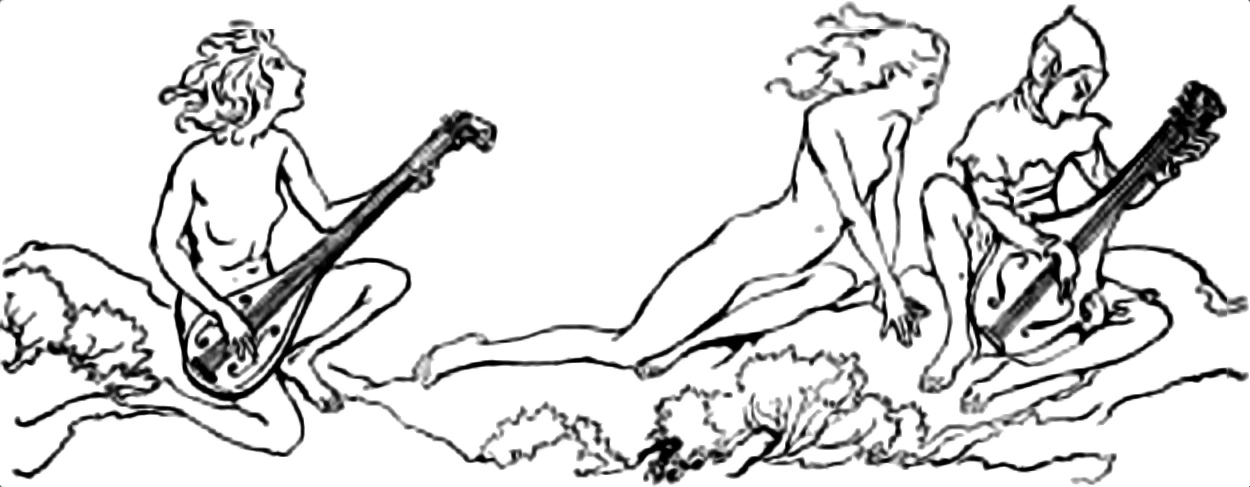
\includegraphics[width=.6\textwidth]{luteborder}
\end{figure}


\begin{verse_speech}[Ferdinand] 
\hspace{\widthof{But certainly a maid.}}My language! heavens!\\
I am the best of them that speak this speech,\\
Were I but where 'tis spoken.
\end{verse_speech}

\begin{verse_speech}[Prospero] 
\hspace{\widthof{Were I but where 'tis spoken.}}How? the best?\\
What wert thou, if the King of Naples heard thee?
\end{verse_speech}

\begin{verse_speech}[Ferdinand] 
A single thing, as I am now, that wonders\\
To hear thee speak of Naples. He does hear me;\\
And that he does I weep: myself am Naples,\\
Who with mine eyes, never since at ebb, beheld\\
The king my father wreck'd.
\end{verse_speech}

\begin{pictures} % This music crept by me upon the waters - letter
	\begin{letter}
		\begin{colorbigpic}
			[1.1]
			{1ii_waters}
			{This music crept by me upon the waters}
		\end{colorbigpic}
	\end{letter}
\end{pictures}


\begin{a4}
	\begin{figure}[tb]
		\centering
		
\includegraphics[width=\textwidth]{grotesque}
	\end{figure}
\end{a4}



\verseline[Miranda]{\hspace{\widthof{The king my father wreck'd.}}Alack, for mercy!}
	
\begin{verse_speech}[Ferdinand] 
Yes, faith, and all his lords; the Duke of Milan\\
And his brave son being twain.
\end{verse_speech}


\begin{pictures} % This music crept by me upon the waters - a4
	\begin{a4}
		\begin{colorbigpic}
			[1.0]
			{1ii_waters}
			{This music crept by me upon the waters}
		\end{colorbigpic}
	\end{a4}
\end{pictures}



\begin{verse_speech}[Prospero] \aside{\hspace{\widthof{And his brave son being twain.}-\widthof{[Aside]}}The Duke of Milan\\
And his more braver daughter could control thee,\\
If now 'twere fit to do't. At the first sight\\
They have changed eyes. Delicate Ariel,\\
I'll set thee free for this.}
\stage{To \textsc{Ferdinand}}
\hspace{\widthof{I'll set thee free for this.}}A word, good sir;\\
I fear you have done yourself some wrong: a word.
\end{verse_speech}

\begin{verse_speech}[Miranda] 
Why speaks my father so ungently? This\\
Is the third man that e'er I saw, the first\\
That e'er I sigh'd for: pity move my father\\
To be inclined my way!
\end{verse_speech}

\begin{verse_speech}[Ferdinand] 
\hspace{\widthof{To be inclined my way!}}O, if a virgin,\\
And your affection not gone forth, I'll make you\\
The queen of Naples.
\end{verse_speech}

\begin{verse_speech}[Prospero] 
\hspace{\widthof{The queen of Naples.}}Soft, sir! one word more.\\
\aside{They are both in either's powers; but this swift business\\
I must uneasy make, lest too light winning\\
Make the prize light.}
\stage{To \textsc{Ferdinand}}
\hspace{\widthof{Make the prize light.}}One word more; I charge thee\\
That thou attend me: thou dost here usurp\\
The name thou owest not; and hast put thyself\\
Upon this island as a spy, to win it\\
From me, the lord on't.
\end{verse_speech}

\verseline[Ferdinand]{\hspace{\widthof{From me, the lord on't.}}No, as I am a man.}
	
\begin{verse_speech}[Miranda] 
There's nothing ill can dwell in such a temple:\\
If the ill spirit have so fair a house,\\
Good things will strive to dwell with't.
\end{verse_speech}

\begin{verse_speech}[Prospero] 
\stage{To \textsc{Ferdinand}}
\hspace{\widthof{Good things will strive to dwell with't.}}Follow me.\\
\stage{To \textsc{Miranda}}

Speak not you for him; he's a traitor. \\
\stage{To \textsc{Ferdinand}}


\hspace{\widthof{Speak not you for him; he's a traitor.}}Come;\\
I'll manacle thy neck and feet together:\\
Sea-water shalt thou drink; thy food shall be\\
The fresh-brook muscles, wither'd roots and husks\\
Wherein the acorn cradled. Follow.\\
\end{verse_speech}

\begin{verse_speech}[Ferdinand] 
\hspace{\widthof{Wherein the acorn cradled. Follow.}}No;\\
I will resist such entertainment till\\
Mine enemy has more power.
\end{verse_speech}

\stage{He draws, and is charmed from moving}


\begin{pictures} % Full fathom five - letter
	\begin{letter}
		\begin{colorbigpic}
			[1.1]
			{1ii_fullfathomfive}
			{Full fathom five thy father lies}
		\end{colorbigpic}
	\end{letter}
\end{pictures}
	





\begin{verse_speech}[Miranda] 
\hspace{\widthof{Mine enemy has more power.}}O dear father,\\
Make not too rash a trial of him, for\\
He's gentle and not fearful.
\end{verse_speech}


\begin{pictures} % Full fathom five - a4
	\begin{a4}
		\begin{colorbigpic}
			[1.0]
			{1ii_fullfathomfive}
			{Full fathom five thy father lies}
		\end{colorbigpic}
	\end{a4}
\end{pictures}
	


\begin{verse_speech}[Prospero] 
\hspace{\widthof{He's gentle and not fearful.}}What? I say,\\
My foot my tutor? Put thy sword up, traitor;\\
Who makest a show but darest not strike, thy conscience\\
Is so possess'd with guilt: come from thy ward,\\
For I can here disarm thee with this stick\\
And make thy weapon drop.
\end{verse_speech}

\verseline[Miranda]{\hspace{\widthof{And make thy weapon drop.}}Beseech you, father.}

\begin{a4}
	\begin{figure}[tb]
		\centering
		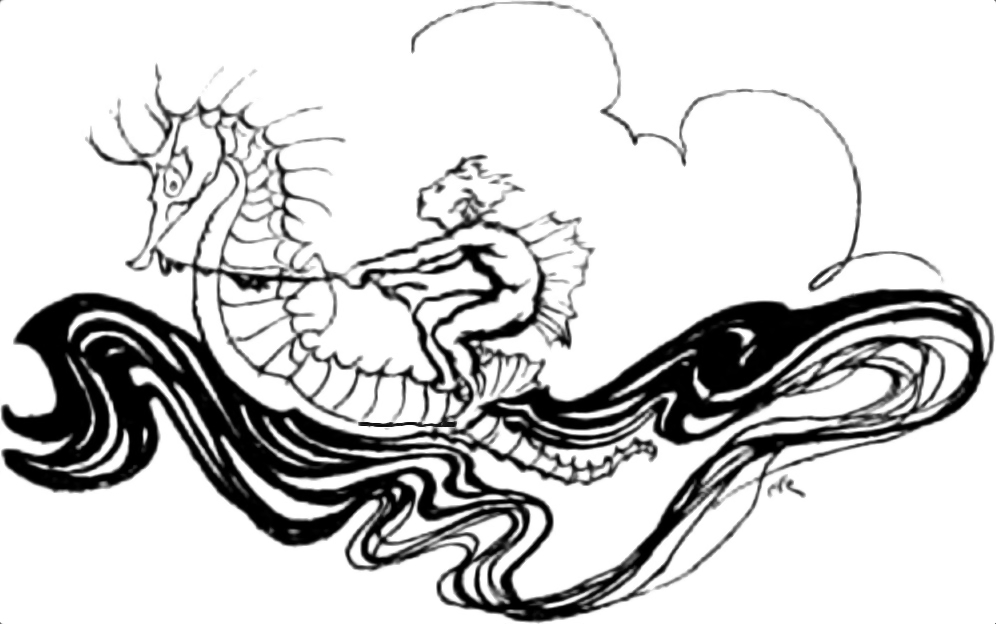
\includegraphics[width=.5\textwidth]{seahorserider}
	\end{figure}
\end{a4}
	
\verseline[Prospero]{Hence! hang not on my garments.}
	
\begin{verse_speech}[Miranda] 
\hspace{\widthof{Hence! hang not on my garments.}}Sir, have pity;\\
I'll be his surety.
\end{verse_speech}

\begin{verse_speech}[Prospero] 
\hspace{\widthof{I'll be his surety.}}Silence! one word more\\
Shall make me chide thee, if not hate thee. What!\\
An advocate for an imposter! hush!\\
Thou think'st there is no more such shapes as he,\\
Having seen but him and Caliban: foolish wench!\\
To the most of men this is a Caliban\\
And they to him are angels.
\end{verse_speech}

\begin{verse_speech}[Miranda] 
\hspace{\widthof{And they to him are angels.}}My affections\\
Are then most humble; I have no ambition\\
To see a goodlier man.
\end{verse_speech}

\begin{verse_speech}[Prospero] 
	\stage{To \textsc{Ferdinand}}
\hspace{\widthof{To see a goodlier man.}}Come on; obey:\\
Thy nerves are in their infancy again\\
And have no vigour in them.
\end{verse_speech}

\begin{verse_speech}[Ferdinand] 
\hspace{\widthof{And have no vigour in them.}}So they are;\\
My spirits, as in a dream, are all bound up.\\
My father's loss, the weakness which I feel,\\
The wreck of all my friends, nor this man's threats,\\
To whom I am subdued, are but light to me,\\
Might I but through my prison once a day\\
Behold this maid: all corners else o' the earth\\
Let liberty make use of; space enough\\
Have I in such a prison.
\end{verse_speech}

\begin{verse_speech}[Prospero] \aside{\hspace{\widthof{Have I in such a prison.}-\widthof{[Aside]}}It works.}
\stage{To \textsc{Ferdinand}}
\hspace{\widthof{Have I in such a prison. It works.}-\widthof{[Aside]}}Come on.\\
Thou hast done well, fine Ariel!
\stage{To \textsc{Ferdinand}}
Follow me.
\stage{To \textsc{Ariel}}
Hark what thou else shalt do me.
\end{verse_speech}

\begin{verse_speech}[Miranda] 
Be of comfort;\\
My father's of a better nature, sir,\\
Than he appears by speech: this is unwonted\\
Which now came from him.
\end{verse_speech}

\begin{verse_speech}[Prospero] 
Thou shalt be free\\
As mountain winds: but then exactly do\\
All points of my command.
\end{verse_speech}

\verseline[Ariel]{To the syllable.}

\verseline[Prospero]{Come, follow. Speak not for him.}
\exeunt{}


\begin{letter}
	\begin{tikzpicture}[remember picture, overlay]
		\node (img) at ($(current page.south)+(0cm,4cm)$) {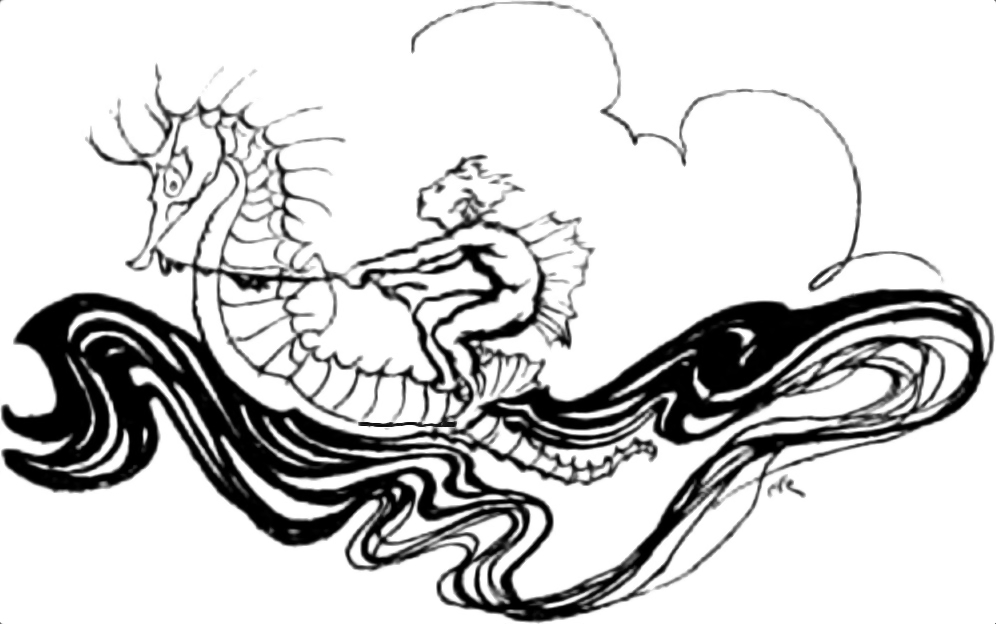
\includegraphics[width=.55\textwidth]{seahorserider}};
	\end{tikzpicture}
\end{letter}
\begin{a4}
	\begin{tikzpicture}[remember picture, overlay]
		\node (img) at ($(current page.south)+(0cm,7cm)$) {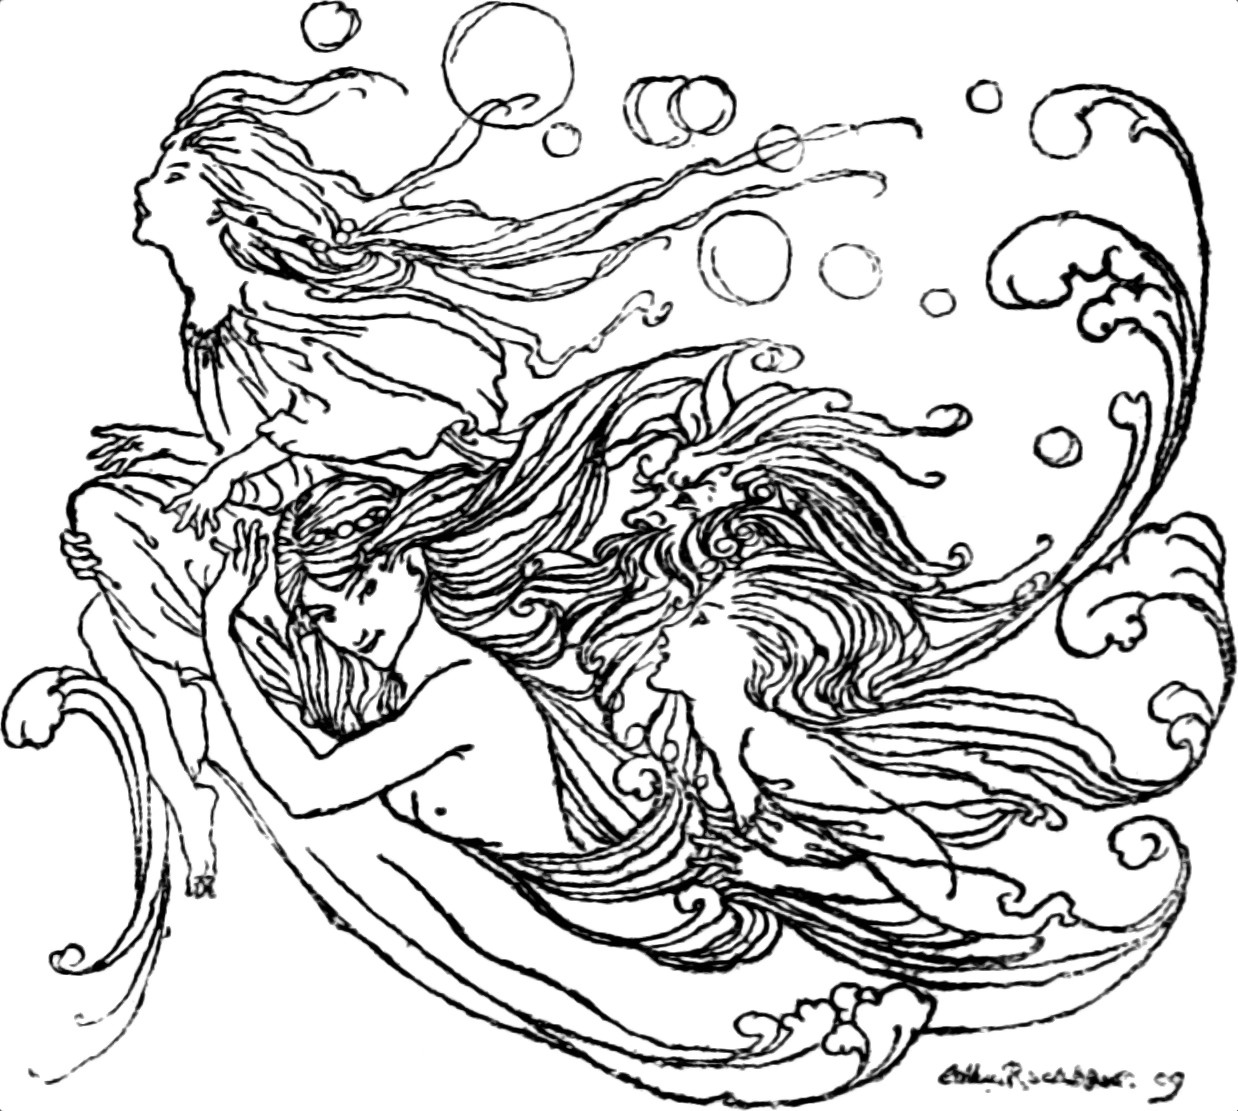
\includegraphics[width=.7\textwidth]{merwave}};
	\end{tikzpicture}
\end{a4}





